% Options for packages loaded elsewhere
\PassOptionsToPackage{unicode}{hyperref}
\PassOptionsToPackage{hyphens}{url}
%
\documentclass[
  12pt,
]{article}
\usepackage{lmodern}
\usepackage{amsmath}
\usepackage{ifxetex,ifluatex}
\ifnum 0\ifxetex 1\fi\ifluatex 1\fi=0 % if pdftex
  \usepackage[T1]{fontenc}
  \usepackage[utf8]{inputenc}
  \usepackage{textcomp} % provide euro and other symbols
  \usepackage{amssymb}
\else % if luatex or xetex
  \usepackage{unicode-math}
  \defaultfontfeatures{Scale=MatchLowercase}
  \defaultfontfeatures[\rmfamily]{Ligatures=TeX,Scale=1}
  \setmainfont[]{Times New Roman}
\fi
% Use upquote if available, for straight quotes in verbatim environments
\IfFileExists{upquote.sty}{\usepackage{upquote}}{}
\IfFileExists{microtype.sty}{% use microtype if available
  \usepackage[]{microtype}
  \UseMicrotypeSet[protrusion]{basicmath} % disable protrusion for tt fonts
}{}
\makeatletter
\@ifundefined{KOMAClassName}{% if non-KOMA class
  \IfFileExists{parskip.sty}{%
    \usepackage{parskip}
  }{% else
    \setlength{\parindent}{0pt}
    \setlength{\parskip}{6pt plus 2pt minus 1pt}}
}{% if KOMA class
  \KOMAoptions{parskip=half}}
\makeatother
\usepackage{xcolor}
\IfFileExists{xurl.sty}{\usepackage{xurl}}{} % add URL line breaks if available
\IfFileExists{bookmark.sty}{\usepackage{bookmark}}{\usepackage{hyperref}}
\hypersetup{
  pdftitle={Migratory shifts in bird abundance along Atlantic Flyway},
  pdfauthor={Cate Jaffe, Emma Wellbaum, Joshua Frear},
  hidelinks,
  pdfcreator={LaTeX via pandoc}}
\urlstyle{same} % disable monospaced font for URLs
\usepackage[margin=2.54cm]{geometry}
\usepackage{graphicx}
\makeatletter
\def\maxwidth{\ifdim\Gin@nat@width>\linewidth\linewidth\else\Gin@nat@width\fi}
\def\maxheight{\ifdim\Gin@nat@height>\textheight\textheight\else\Gin@nat@height\fi}
\makeatother
% Scale images if necessary, so that they will not overflow the page
% margins by default, and it is still possible to overwrite the defaults
% using explicit options in \includegraphics[width, height, ...]{}
\setkeys{Gin}{width=\maxwidth,height=\maxheight,keepaspectratio}
% Set default figure placement to htbp
\makeatletter
\def\fps@figure{htbp}
\makeatother
\setlength{\emergencystretch}{3em} % prevent overfull lines
\providecommand{\tightlist}{%
  \setlength{\itemsep}{0pt}\setlength{\parskip}{0pt}}
\setcounter{secnumdepth}{5}
\ifluatex
  \usepackage{selnolig}  % disable illegal ligatures
\fi

\title{Migratory shifts in bird abundance along Atlantic Flyway}
\usepackage{etoolbox}
\makeatletter
\providecommand{\subtitle}[1]{% add subtitle to \maketitle
  \apptocmd{\@title}{\par {\large #1 \par}}{}{}
}
\makeatother
\subtitle{\url{https://github.com/jofrear/JaffeWellbaumFrear_ENV872_EDA_FinalProject}}
\author{Cate Jaffe, Emma Wellbaum, Joshua Frear}
\date{}

\begin{document}
\maketitle

\newpage
\tableofcontents 
\newpage
\listoftables 
\newpage
\listoffigures 
\newpage

\hypertarget{rationale-and-research-questions}{%
\section{Rationale and Research
Questions}\label{rationale-and-research-questions}}

Bird presence and abundance shifts seasonally for many species in the
US. We wanted to investigate these shifts, both within a year, and
across years, and compare it with temperature data. To do this, we
analyzed citizen-science observations from Ebird of three key bird
species: Pandion haliaetus (Osprey), Aix sponsa (Wood Duck), and
Agelaius phoeniceus (Red-Winged Blackbird). These species from different
orders were selected based on news reports and published papers that
suggested recent shifts in abundance and range.

\newpage

\hypertarget{dataset-information}{%
\section{Dataset Information}\label{dataset-information}}

Bird observation data was downloaded from the Cornell Lab of Orinthology
eBird Database (\url{https://ebird.org/}). Data was obtained for the
three target species in three states along the Atlantic migratory
Flyway: Maine, Massachusetts, and North Carolina. All observations
uploaded to ebird and marked with an observation date between January
2010 and March 2021 were used. Citizen science observers using ebird
enter the bird species seen and numbers observed for each species, and
can optionally track their effort in birding by including distance
traveled during a trip (which can be manually entered or derived from
smartphone gps data) and time spent observing.

\newpage

\hypertarget{exploratory-analysis}{%
\section{Exploratory Analysis}\label{exploratory-analysis}}

It became clear that observations dataset had generally increasing
observations year-over-year, regardless of species (Figure 1). This is
possibly attributable to increasing ebird use in the US, especially as
smartphone adoption increased over the last decade, providing an
electronic alternative to pen-and-paper notations of field observations.

To adjust for this trend, we used the reported time spent observing
birds on each checklist to create a value of observed birds per minute
(Figure 2). The distribution of birds observed per minute was
non-normal, but log-transforming the data revealed a roughly normal
distribution.

\begin{figure}
\centering
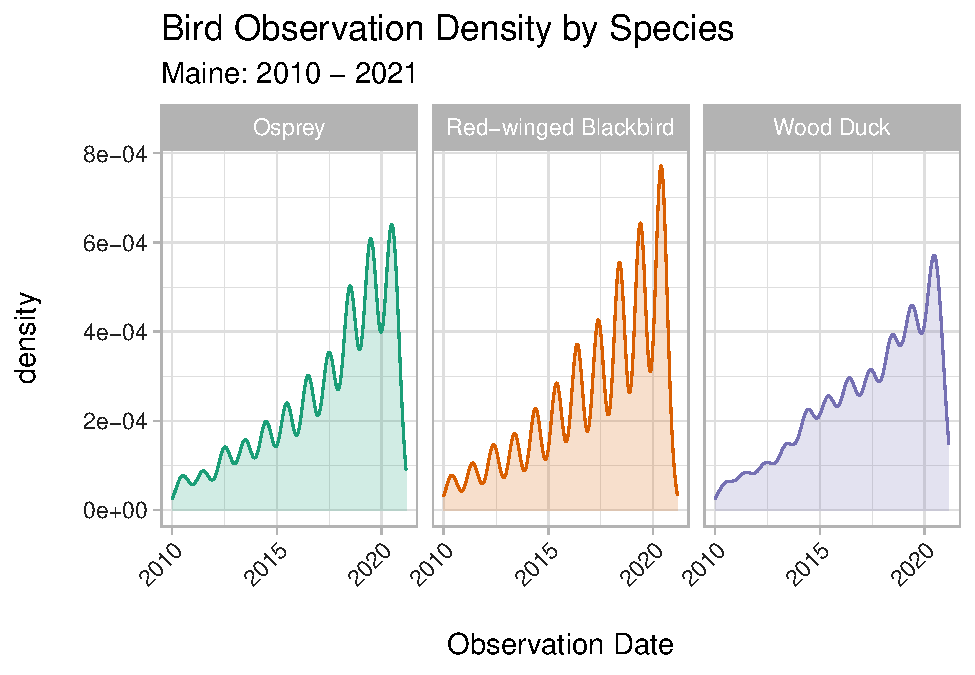
\includegraphics{Project_report_ME_files/figure-latex/density.plot-1.pdf}
\caption{Density of ebird observations in Maine from 2010 - 2021.}
\end{figure}

\begin{figure}
\centering
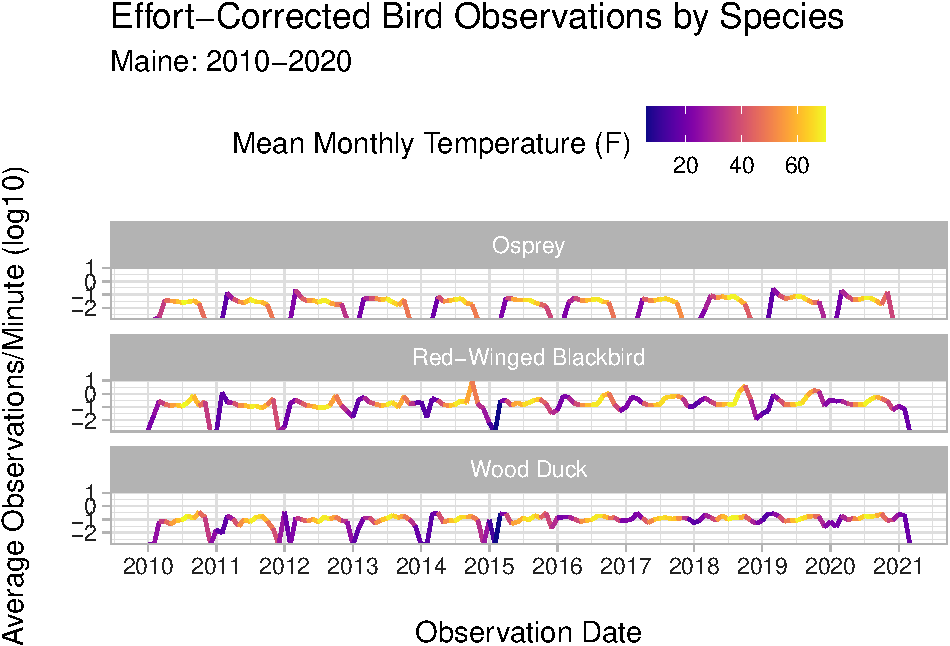
\includegraphics{Project_report_ME_files/figure-latex/monthly.log.effort-1.pdf}
\caption{Bird observations in Maine, grouped by month, adjusted per
minute of observation and log-transformed.}
\end{figure}

\newpage

\hypertarget{analysis}{%
\section{Analysis}\label{analysis}}

Two approaches were taken towards analyzing whether there has a been a
shift in abundance over the study period. The simpler but cruder
approach is to use a linear model with the month of observation as a
continuous variable. When examined this way, Of the three species, only
Wood Ducks showed a statistically significant change in observations per
minute across the study period (slope = 1.289e-05, R\^{}2 = 0.04, p
\textless{} 0.05). This small shift in abundance for Wood Ducks may
indicate increasing abundance, but it does not explain the variance in
the data, likely because seasonal migration patterns are dominant.

The second approach is to construct a time series analysis for the
observations. According to the time series analysis, each of the species
showed both a strong seasonal component in observations, and a rising
monotonic trend across the study period in Maine, according to the
seasonal Mann-Kendall test (Osprey: tau = 0.389, p \textless{} 0.001,
Wood Duck: tau = 0.269, p \textless{} 0.001, Red-Winged Blackbird: tau =
0.335, p \textless{} 0.001) (Figures 3 - 5). This rising trend may be
due to increasing abundance of these species, but it may also be due to
several confounding factors, including variability in observations by
birders (e.g.~location, time of day, or increasing expertise).

Each of the species had an influx of observations associated with spring
migration (Febuary-April). Wood Ducks and Red-Winged Blackbird seasonal
trends revealed two spikes, suggesting that most spring and fall
observations are not from summer residents, but from migrating
individuals from out-of-state. Osprey observations, on the other hand,
had a relatively constant seasonal component for summer and fall.

\begin{figure}
\centering
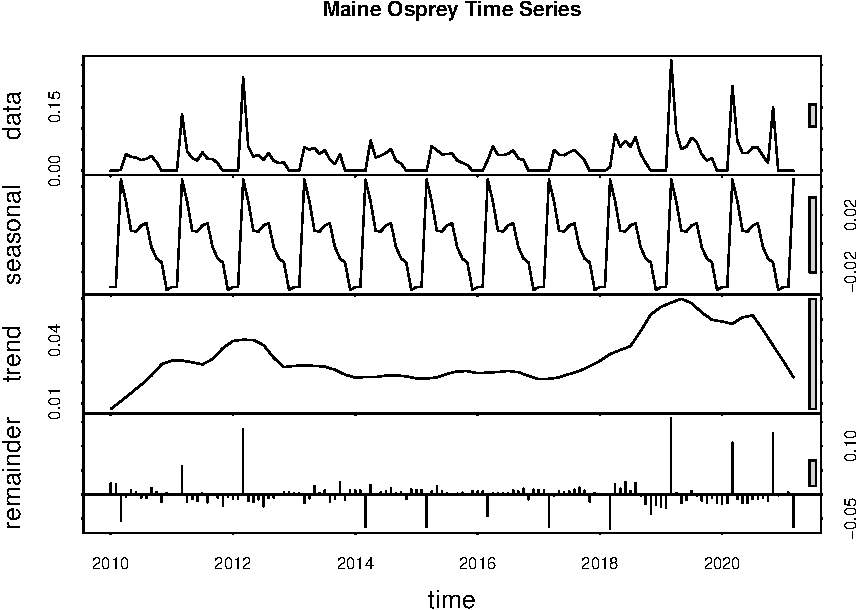
\includegraphics{Project_report_ME_files/figure-latex/Time.SeriesO-1.pdf}
\caption{Time Series of Maine Osprey Observations per Minute,
2010-2021.}
\end{figure}

\begin{figure}
\centering
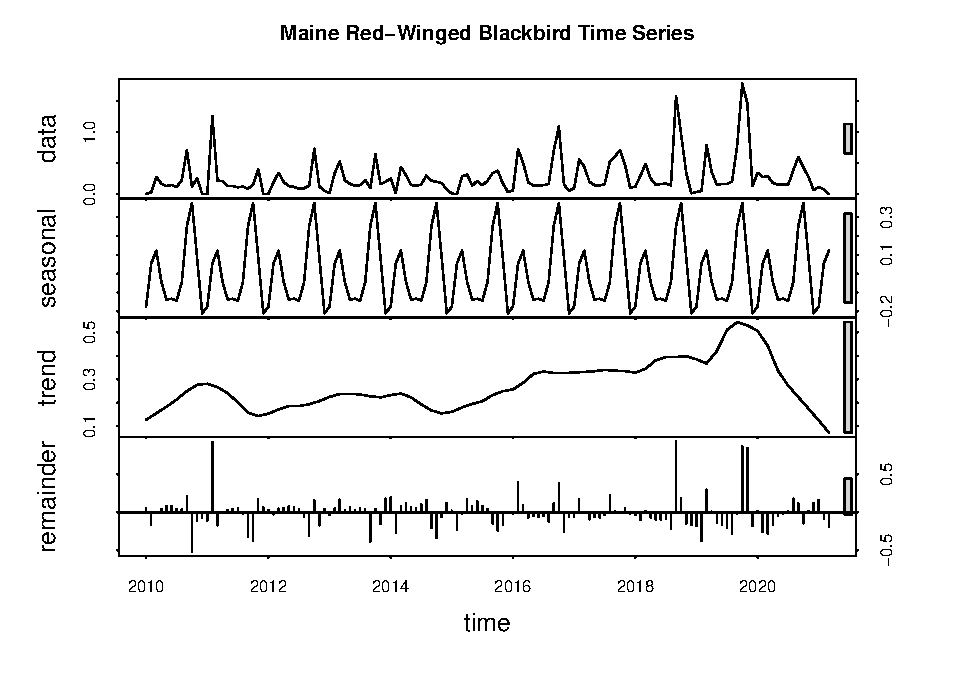
\includegraphics{Project_report_ME_files/figure-latex/Time.SeriesR-1.pdf}
\caption{Time Series of Maine Red-Winged Blackbird Observations per
Minute, 2010-2021.}
\end{figure}

\begin{figure}
\centering
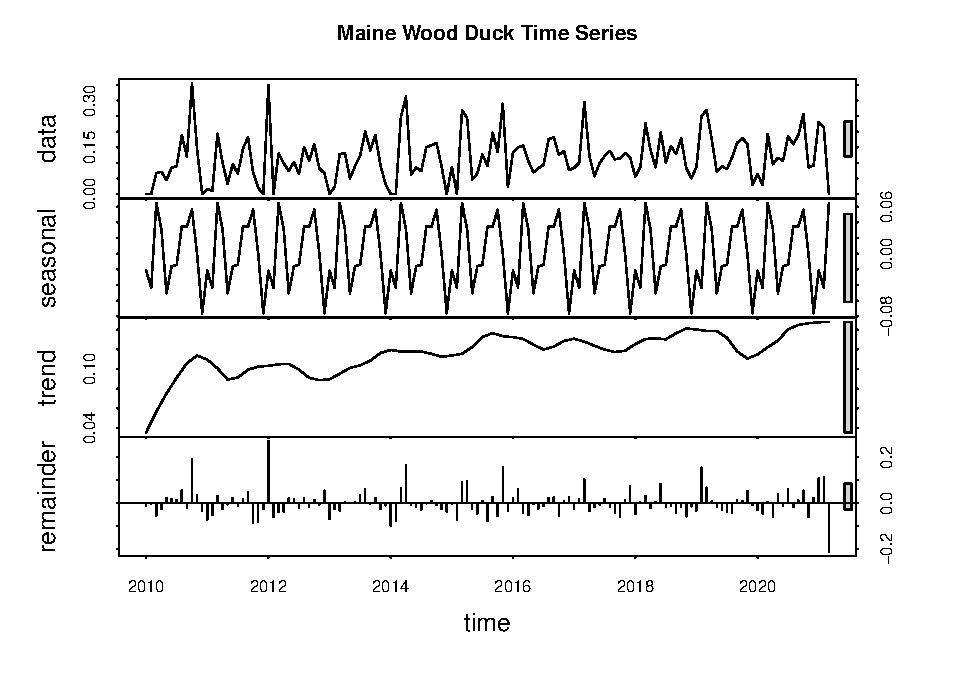
\includegraphics{Project_report_ME_files/figure-latex/Time.SeriesW-1.pdf}
\caption{Time Series of Wood Duck Observations per Minute, 2010-2021.}
\end{figure}

\hypertarget{question-1}{%
\subsection{Question 1:}\label{question-1}}

Are non-migratory populations of a species establishing themselves in
regions that formerly only had migratory populations of that species?

The first step towards answering this question would be the
identification of overwintering individuals - that is, observations of
individuals during the time that migratory populations should be absent
from the region, typically December and January. In Maine, we see
observations of Red-Winged Blackbirds during all months, indicating that
there is a resident population, despite the migratory behavior and
strong seasonal trend. Ospreys are completely absent from Maine for the
winter months, with the latest observations in the 2nd week of November,
and the earliest observations at the end of March.

Wood Ducks, however, present a possible trend. The first 5 winters had
gaps between 33 and 86 days during which no Wood Ducks were observed in
Maine. Beginning in the 2015-2016 winter, the observations gaps
disappeared, with individuals seen on both in the last week of
Decemeber, and first week of January. A small gap did reappear in the
last two winters, with periods of 27 and 13 days in which no individuals
were observed.

\newpage

\hypertarget{summary-and-conclusions}{%
\section{Summary and Conclusions}\label{summary-and-conclusions}}

The Wood Duck data suggests that either birders in Maine are discovering
wintering Wood Ducks that they previously overlooked, or that Wood Ducks
are responding to climate shifts that make certain locations in Maine
suitable wintering habitat. More observations are needed to explore this
trend.

We expect to see significant shifts in bird distribution and abundance
as temperatures rise over this century, particularly in species like
Osprey (Pandion haliaetus) that have both migratory and resident
populations. Populations in regions that are currently migratory (like
those in Massachusetts and Maine) may become year-round residential
populations if the climate facilitates this. The study period of ten
years does not reveal any shifts in seasonality. The first indicators of
a shift like this will likely come in changes to ``first-of-year''
sightings, which are worth monitoring. Migratory species that are unable
to adapt to climate shifts will likely face strong inter-specific
competition from non-migratory species.

\end{document}
